\documentclass{article}
\usepackage[T1]{fontenc}
\usepackage[latin2]{inputenc}
\usepackage[english]{babel}
\usepackage{tikz}
\usetikzlibrary{calc,through,backgrounds,positioning,fit}
\usetikzlibrary{shapes,arrows,shadows}
 
\begin{document}
 
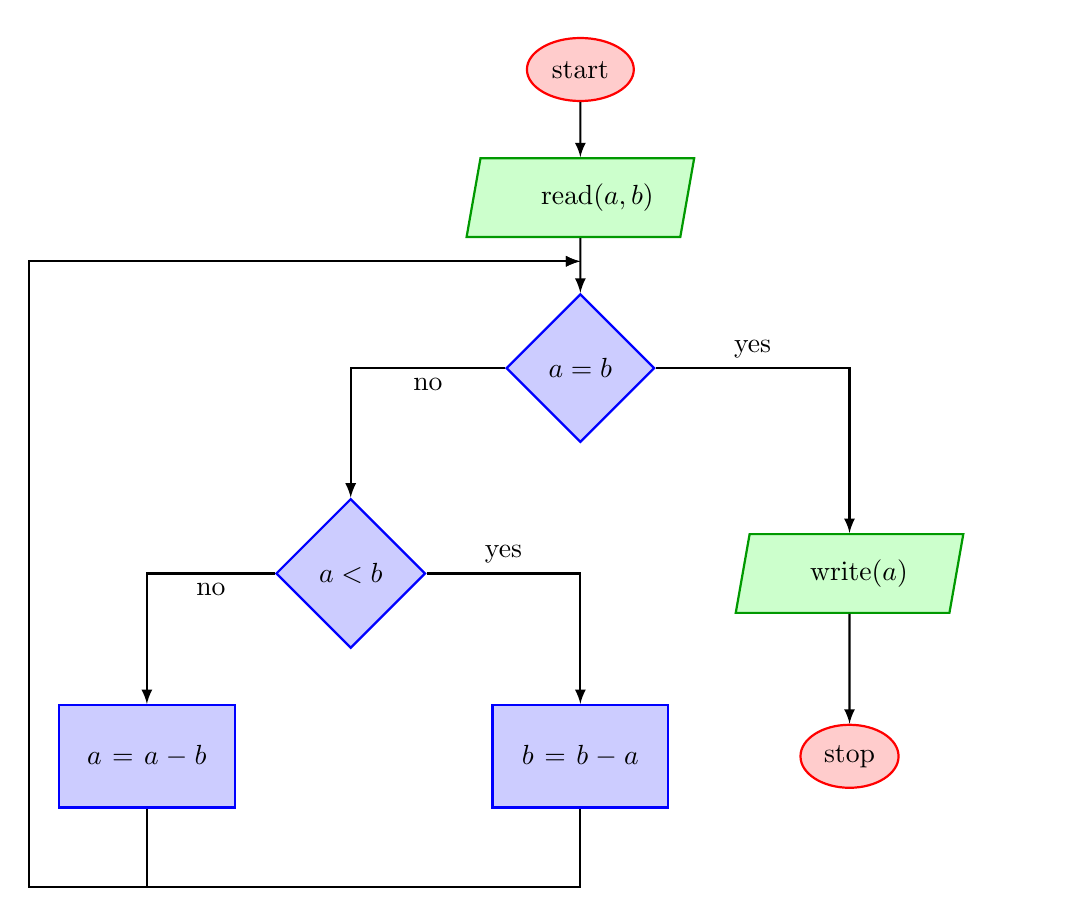
\begin{tikzpicture}[auto,
decision/.style = {diamond, draw=blue, thick, fill=blue!20, text width=1.5cm, 
                   align=flush center, inner sep=1pt},
block/.style = {rectangle, draw=blue, thick, fill=blue!20, text width=2cm, 
                align=center, minimum height=1.3cm},
start/.style = {draw=red, thick, ellipse, fill=red!20, minimum height=8mm},
inout/.style = {draw=green!60!black, thick, fill=green!20, trapezium, trapezium left angle=80, 
                trapezium right angle=-80, minimum height=10mm, text width=1cm, align=center, 
                inner sep=1pt},
line/.style ={draw, thick, -latex}]
 
\matrix[column sep=5mm,row sep=7mm]
{
&& \node [start] (start) {start}; & \\
&& \node [inout] (read) {read($a,b$)}; & \\
&& \node [decision] (decide) {$a=b$}; & \\
&\node [decision] (decide2) {$a<b$};  &&
\node [inout] (write) {write($a$)}; \\
\node [block] (block) {$a=a-b$}; &&
\node [block] (block2) {$b=b-a$};
& \node [start] (stop2) {stop}; &&\\
};
 
\begin{scope}[every path/.style=line]
\path (start) -- (read);
\path (read) -- (decide);
\path (decide) -| node [near start] {yes} (write);
\path (decide) -| node [near start] {no} (decide2);
\path (decide2) -| node [near start] {yes} (block2);
\path (decide2) -| node [near start] {no} (block);\\
\path (write) -- (stop2);
\path (block.south) -- ++(0,-1) -- ++(-1.5,0) |- ($ (decide.north) + (0,0.4) $);
\path (block2.south) -- ++(0,-1) -- ++(-7,0) |- ($ (decide.north) + (0,0.4) $);
\end{scope}
\end{tikzpicture}
\end{document}